\chapter{Future work}
This PhD provides a snapshot of research I have done in recent years. This work fits within a larger body of research with similar overall objectives, to improve both the software and how that software is developed. This chapter introduces various topics related to my ongoing research which may be of interest to the research community.

\section{Evaluating Google Play Console Reports}
With discovering the many and various flaws and quirks in Google's analytics products I decided a set of experiments would help increase the trust and transparency of Android Vitals and Google Play Console. Aspects of these experiments may also be highly relevant to evaluate other analytics tools, products, and services. Some of the experiments could trigger defensive mechanisms used to 'protect' large-scale online services such as Google Play. For instance App Stores, including Google Play, are known to take protective and corrective activities related to fake reviews. Some experiments might want to assess the effectiveness of protective defenses, others may aim to avoid triggering them. 

Google is known to take punitive actions against developers whom it deems to be related to undesirable behaviours. %MUST-DO add references to examples. 
As these actions can include a lifetime ban for the account deemed to have transgressed, and for other accounts it considers are related, the effects of their actions can be far reaching and remove all revenues for an organisation's Android apps where the onus is on the people in that organisation being able to convince Google of the merits of reinstatement often without knowing what the reasons were, what the evidence was, and with no other practical way of restoring their account.

The Google Engineering team have been defensive and guarded in terms of suggestions to help evaluate the behaviours of their system. SHOULD-DO add some examples. 

A cautious set of basic tests to help establish characteristics of analytics from no (zero) to tens of users is available online at 
\url{https://joedocs.com/julianharty/evaluating-gpc-reports}

\textbf{Placeholders to extend on this topic}: Holding ourselves and each other to account. Humility, openness, comparisons with financial auditing of businesses. \emph{c.f.} Sentry.io's work, opensourcing of client libraries, etc. 

\begin{itemize}
    \item Due diligence. \emph{`Trust and Confirm')~\footnote{\url{https://www.leadergrow.com/articles/443-trust-but-verify}}}. The risks of overtrusting and not doing due diligence, especially where money is involved. The author encourages verification (as I do). Beware of end to end systems that are not verifiable by an outside party~\footnote{\url{https://www.forbes.com/sites/frankarmstrong/2019/10/21/trust-but-verify/}}.
    \item \emph{``The Only Thing Necessary for the Triumph of Evil is that Good Men Do Nothing"}~\footnote{\url{https://quoteinvestigator.com/2010/12/04/good-men-do/}}
\end{itemize}

\section{Research into Google Android data collection}
The mechanism(s) Google uses to collect data on devices is worthy of research given the scope, range and effects of this data in terms of assessing qualities of all the Android apps in Google Play.

My work has identified numerous flaws in the reporting, do any of these stem from the data collection on the devices? Is it possible? is it practical? to generate fake data that Google would use and rely on? Research has already found evidence of systemic tainting of ratings and reviews, perhaps it's also possible that diagnostic and usage data can also be tainted at scale?

related work: Botnets, black market reviews, device farms using emulators, device farms intended for testing, ...

A related topic is to better understand whether the underlying device data can be accessed using non-Google software. 

\begin{enumerate}
    \item What data does Android Vitals capture?
    \item Where is that data available on Android devices?
    \item Ways to access that data?
    \item Homebrew approach to accessing, collecting, and analysing the data.
\end{enumerate}

\subsection{Homebrew}
As discussed in section \href{platform-level-analytics}{\emph{\nameref{platform-level-analytics}}}, parsing the Android logs requires Android permission(s) ... Once the software has been granted permission it can read all the logs (...) and parse them. [Presumably] the logs are read-only for apps (the history can be cleared using the \texttt{adb logcat} command-line command externally (e.g. from a PC).

Structure and presentation of content in the Android logs: ...
Consistency in pertinent events in Android logs (we believe they're consistently formatted with predictable elements always provided, which makes them easier to parse and process).



\section{Enhancing quality vs. enhancing UX}\label{enhancing-quality-vs-enhancing-ux}
Success of software is multifactorial and development teams need to consider where, when and how to focus their energies to achieve satisfactory outcomes for themselves and their patrons (often their management and funders). Where does improving and achieving high-quality software fit amongst other demands on their time and energies?

\begin{figure}[ht]
    \centering
    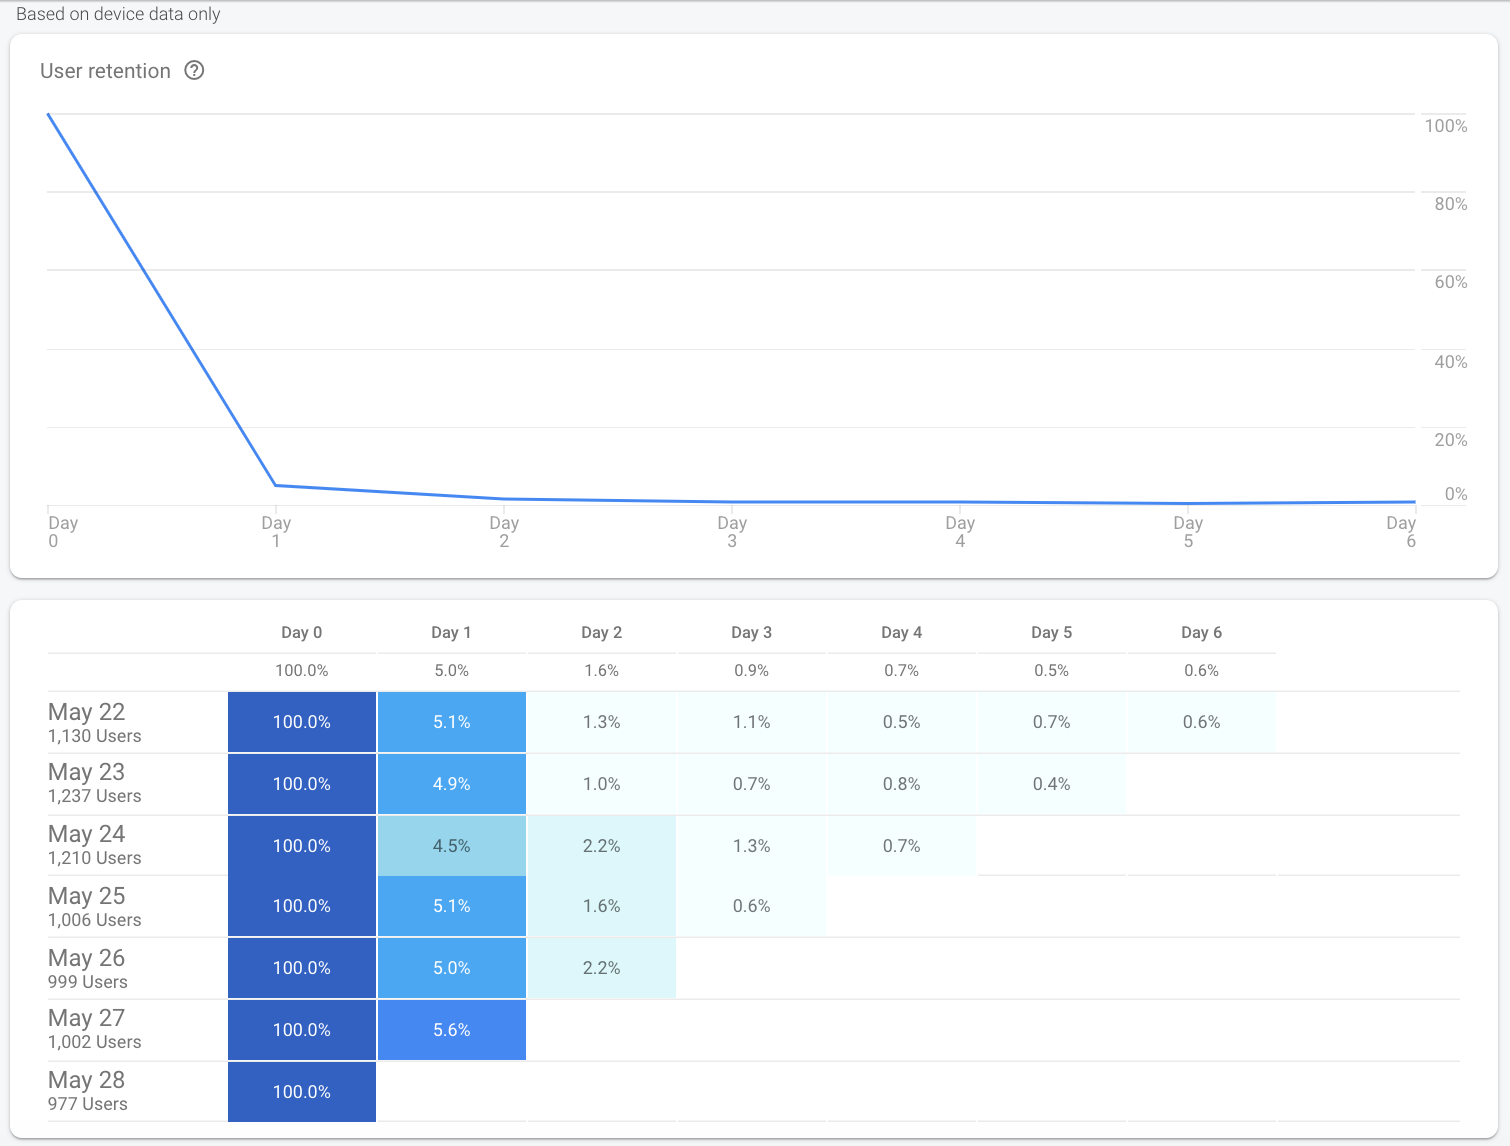
\includegraphics[width=10cm]{images/firebase/Firebase-pocketcode-android-7-day-new-user-retention-29-may-2020.png}
    \caption{Firebase>Catrobat>New User Retention}
    \label{fig:Firebase-pocketcode-android-7-day-new-user-retention-29-may-2020}
\end{figure}

An area of my ongoing research is to evaluate the impacts of enhancing software quality in terms of stability compared to enhancing the UX of an app. The Pocket Code mobile Android app has low retention rates for new users according to Firebase, the 7 day retention of new users is illustrated in Figure \ref{fig:Firebase-pocketcode-android-7-day-new-user-retention-29-may-2020}. Both the iOS and Android Pocket Code apps have similar screens, especially the initial screens seen by new users of either app. Through our research and the focus on identifying and fixing various stability metrics we plan to focus on improving the design of the user experience for new users. One measure will be the `new user retention' report.

\section{Adding in-app analytics to PocketCode}
The Pocket Code Android app included the legacy Fabric Crashlytics analytics library for several years predating my involvement with the project (the earliest commit to add Fabric Crashlytics is on \nth{27} June 2017~\footnote{\href{https://github.com/Catrobat/Catroid/commit/95aa37ff5263402b41b63f50296aabc8c354433e}{\texttt{CAT-2420 Replace Firebase with Crashlytics}}}). This recorded both caught and uncaught exceptions but nothing else about how the app was used, or by whom. As part of my collaboration with the Catrobat team we agreed we would design and add in-app analytics in addition to the crash reporting. This work coincided with migrating from the legacy Fabric reports to the replacement Firebase reports so Firebase Analytics was selected. I helped lead the initial design and testing of the in-app analytics~\footnote{Various details are available in a Google hosted document~\url{https://docs.google.com/document/d/1cqCP2aqcx8mpTTHWe9ooGygtXh7eTvYzM3f9FbexUNM/edit?usp=sharing}}. The work has been delayed because of various impacts of the COVID-19 pandemic, the aim is to resume it as various countries and regions emerge from their respective lockdowns.

\section{Developer-centric logging in mobile apps}
Developers use logging for various reasons when they work with source code. Therefore developers use logging when they work on source code for mobile apps. Do they use logging in particular ways or for specific purposes when developing mobile apps? Research considerations include the use of remote logging and/or the use of mobile analytics.

My research in mobile analytics overlaps and closely aligns with research on logging - both are used by software development teams to learn about how their software behaves. I am part of a group of distributed, international researchers investigating aspects of how and why developers add logging to their mobile applications. One of our current research areas investigates the use of Google Firebase Analytics for logging. \emph{Ad-hoc} research notes are available at \url{https://joedocs.com/julianharty/apm-logging-research}.


\section{Improving the design, implementation and engineering of in-app analytics}
Research in approaches to improve the design, implementation and engineering of in-app analytics may inform the state of the art in the use of in-app analytics, particularly for software engineering and software quality. It may also help inform and guide the practice of in-app analytics. 

Commercial services, such as \href{http://iterative.ly}{Iteratively}, aim to facilitate the \emph{``capture [of] accurate analytics right firs time"} and enable developers to \emph{``Quickly instrument analytics with code snippets and automated QA."} through their software tools. How might services such as these help development teams improve their engineering of in-app analytics? 

Two suggested areas of research are whether these tools successfully guide developers to:
\begingroup
\renewcommand{\theenumi}{\alph{enumi}}
\begin{enumerate}
    \item actively use data already available to them?
    \item design how to use optional analytics tools efficaciously?
\end{enumerate}
\endgroup
% Thanks to: https://tex.stackexchange.com/questions/346787/how-can-i-get-a-list-starting-with-a-b-c-instead-of-1-2-3

\section{Dynamic Adaptive logging in mobile apps}
This is a placeholder and a reminder to incorporate some early ideas on this topic in an unpublished paper titled \emph{``Dynamic Distributed Logging and Analytics"}, see \url{https://www.overleaf.com/read/mgcrcqkbsnzh}.

\section{Using Mobile Analytics to improve testing of mobile apps}
% MUST-DO expand this section.
\begin{itemize}
    \item Using Mobile Analytics to improve the testing of mobile apps. This was work I had hoped to perform as part of this research, various practical constraints meant this was not practical during the PhD.
\end{itemize}

\section{Digital twins for software apps}
Digital twins are variously defined as \emph{``a high-fidelity digital model of a physical system or asset that can be used e.g. to optimize operations and predict faults of the physical system."}~\cite{pokhrel2020_digitaltwin_for_cybersecurity} and \emph{``Digital twins integrate IoT, artificial intelligence, machine learning and software analytics with spatial network graphs"}~\cite{wikipedia__digital_twin} (attributed to Microsoft in 2018 in the Wikipedia article). Twins have been used for various engineering challenges including jet turbine performance engineering and may help transform the engineering lifecycle for many products, including jet turbines~\cite{read2018_digital_takeover_avionics}, cars. As~\cite{pokhrel2020_digitaltwin_for_cybersecurity} observes, digital twins may also represent cyber-security and potentially humble, mobile apps.

``A Digital Twin will continuously learn and update itself using data from sensors that monitor various aspects of the real-life product’s environment and operating conditions. It can also factor in historical data from prior usage."~\url{https://www.rolls-royce.com/media/our-stories/discover/2019/how-digital-twin-technology-can-enhance-aviation.aspx}
% https://www.aerospacetechreview.com/twinning-digital-twins-show-their-power-by-louise-bonnar/

A digital twin for mobile apps is likely to include controlled run-time environments including high-fidelity emulators and physical devices since some problems and behaviours may be triggered and/or exposed by particular run-time environment. Mobile Analytics may help inform the selection of run-time environment as well as the identification of software quality concerns. As mobile apps are increasingly used in very sensitive and critical environments where the consequences are material, digital twins may also be used to validate the behaviours and outputs of the apps for end users.

% https://golden.com/wiki/Digital_twin-6MX6WP % repeats the definition from Wikipedia that apparently came from MSFT in 2018.

\section{Summary of Future Work}
The thesis is a snapshot of work done to date. The PhD journey and a combination of the relationships and experiences that have been established on the journey have led to various interesting and related areas of ongoing and future work which I am actively engaged in. Please get in contact if you would like to collaborate with any of these and/or with other topics that relate to my research.
